%!TEX root = ../bug-taxo.tex


\subsection{Version control systems\label{sec:version-control}}

Version control consists of maintaining the versions of files --- such as source code and other software artifacts \cite{Zeller1997}.
This activity is a complex task and cannot be performed manually on real world project.
Consequently, numerous tools have been created to help practitioners manage the version of their software artifacts.
Each evolution of a software is a version (or revision) and each version (revision) is linked to the one before through modifications of software artifacts.
These modifications consist of updating, adding or deleting software artifacts.
They can be referred as \texttt{diff}, {\tt patch} or {\tt commit}\footnote{These names are not to be used interchangeably as difference exists.}.
Each \texttt{diff}, {\tt patch} or {\tt commit} have the following characteristics:

\begin{itemize}
\item Number of Files: The number of software files that have been modified, added or deleted.
\item Number of Hunks: The number of consecutive code blocks of modified, added or deleted lines in textual files. Hunks are used to determine, in each file, how many different places the developer has modified.
\item Number of Churns:  The number of lines modified. However, the churn value for a line change should be at least two as the line has to be deleted first and then added back with the modifications.
\end{itemize}

In modern versioning systems, when maintainers make modifications to the source code want to version it, they have to do commit.
The commit operation will version the modifications applied to one or many files.

Figure \ref{fig:branching} presents the data structure used to store a commit.
Each commit is represented as a tree.
The root leaf (green) contains the commit, tree and parent hashes as same as the author and the description associated with the commit.
The second leaf (blue) contains the leaf hash and the hashes of the files of the project.

\begin{figure}[h!]
  \centering
    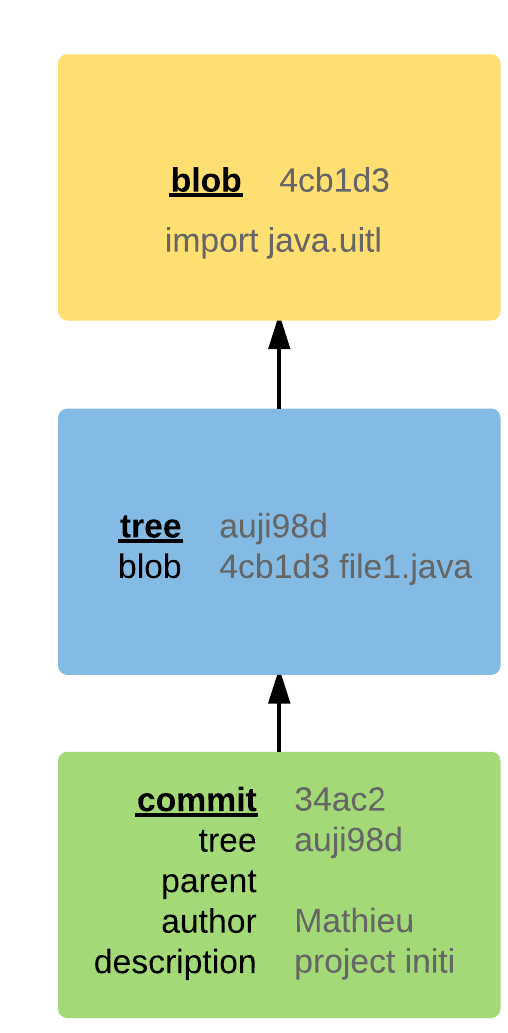
\includegraphics[scale=0.20]{media/commit-datastructure.png}
    \caption{Data structure of a commit.
    \label{fig:branching}}
\end{figure}

In this example, we can see that author ``Mathieu'' has created the file $file1.java$ with the message ``project init''.

\subsection{Project Tracking Systems\label{sec:issue-tracking}}

Project tracking systems allow end users to create bug reports (BRs) to report unexpected system behavior,
manager can create tasks to drive the evolution forward and crash report (CRs) can be automatically created.
These systems are also used by development teams to keep track of the modification induced by bug and to crash reports, and keep track of the fixes.

\begin{figure}[h!]
	\centering
	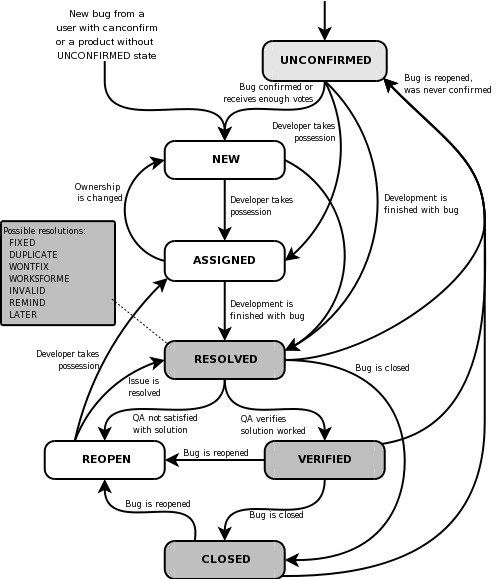
\includegraphics[scale=0.5]{media/bzLifecycle.png}
	\caption{Lifecyle of a report \cite{Bugzilla2008}}
	\label{fig:bug-lifecyle}
\end{figure}

Figure \ref{fig:bug-lifecyle} presents the life cycle of a report.
When a report is submitted by an end-user, it is set to the {\tt UNCONFIRMED} state until it receives enough votes or that a user with the proper permissions modifies its status to {\tt NEW}.
The report is then assigned to a developer to be fixed.
When the report is in the {\tt ASSIGNED} state, the assigned developer(s) starts working on the report.
A fixed report moves to the {\tt RESOLVED} state. Developers have five different possibilities to resolve a report: {\tt FIXED}, {\tt DUPLICATE}, {\tt WONTFIX}, {\tt WORKSFORME} and {\tt INVALID} \cite{Koponen2006}.

\begin{itemize}
	\item {\tt RESOLVED/FIXED}: A modification to the source code has been pushed, i.e., a changeset (also called a patch) has been committed to the source code management system and fixes the root problem described in the report.
	\item {\tt RESOLVED/DUPLICATE}: A previously submitted report is being processed. The report is marked as duplicate of the original report.
	\item {\tt RESOLVED/WONTFIX}: This is applied in the case where developers decide that a given report will not be fixed.
	\item {\tt RESOLVED/WORKSFORME}: If the root problem described in the report cannot be reproduced on the reported OS / hardware.
	\item {\tt RESOLVED/INVALID}: If the report is not related to the software itself.
\end{itemize}

Finally, the report is {\tt CLOSED} after it is resolved.
A report can be reopened (sent to the {\tt REOPENED} state) and then assigned again if the initial fix was not adequate (the fix did not resolve the problem).
The elapsed time between the report marked as the new one and the resolved status are known as the {\it fixing time}, usually in days.
In case of task branching, the branch associated with the report is marked as ready to be merged.
Then, the person in charge (quality assurance team, manager, ect...) will be able to merge the branch with the mainline.
If the report is reopened: the days between the time the report is reopened and the time it is marked again as {\tt RESOLVED/FIXED} are cumulated.
Reports can be reopened many times.

Tasks follow a similar life cycle with the exception of the {\tt UNCONFIRMED} and {\tt RESOLVED} states.
Tasks are created by management and do not need to be confirmed in order to be {\tt OPEN} and {\tt ASSIGNED} to developers.
When a task is complete, it will not go to the {\tt RESOLVED} state, but to the {\tt IMPLEMENTED} state.
Bug and crash reports are considered as problems to eradicate in the program.
Tasks are considered as new features or amelioration to include in the program.

Reports and tasks can have a severity\cite{Bettenburg2008}.
The severity is a classification to indicate the degree of  impact on the software.
The possible severities are:

\begin{itemize}
	\item blocker: blocks development and/or testing work.
	\item critical: crashes, loss of data, severe memory leak.
	\item major: major loss of function.
	\item normal: regular report, some loss of functionality under
 specific circumstances.
  \item minor: minor loss of function, or other problem where easy workaround is present.
	\item trivial: cosmetic problems like misspelled words or misaligned text.
\end{itemize}

The relationship between an report or a task and the actual modification can be hard to establish and it has been a subject of various research studies (e.g., \cite{Antoniol2002,Bachmann2010,Wu2011}).
This reason is that they are in two different systems: the version control system and the project tracking system.
While it is considered a good practice to link each report with the versioning system by indicating the report $\#id$ on the modification message, more than half of the reports are not linked to a modification\cite{Wu2011}.
